\documentclass[a4paper,landscape,12pt]{article}
\usepackage[svgnames]{xcolor}
\usepackage{adjustbox}
\usepackage{wallpaper}
\usepackage{ragged2e}
\usepackage{ulem}
\usepackage{graphicx}
\usepackage{etoolbox}
\usepackage[object=pgfhan]{pgfornament}
\usetikzlibrary{chains}
\usetikzlibrary{calc}
\usetikzlibrary{decorations}
\usetikzlibrary{decorations.text,decorations.markings}
\usetikzlibrary{decorations.pathmorphing,shadows}

\usepackage{geometry}
\geometry{hmargin=1in,vmargin=0.8in,headheight=25pt}

\usepackage{fancyhdr}
\fancyhf{}
\renewcommand{\headrule}{}

\newpgfornamentfamily{pgfhan}
\newbox{\fortyseven}
\savebox{\fortyseven}{
    \tikzset{every node/.append style={inner sep=0pt,color=MidnightBlue!50}}
    \tikzset{pgfornamentstyle/.style={draw=green!20!black,
    fill=orange,fill opacity=.5,thick}}%
\pgfornament[scale=0.50]{32}}

\newbox{\myfancyhead}
\AtBeginDocument{
\savebox{\myfancyhead}{
\newpgfornamentfamily{pgfhan}
\begin{tikzpicture}[overlay,remember picture]
    \tikzset{every node/.append style={inner sep=0pt,color=MidnightBlue!50}}
    \tikzset{pgfornamentstyle/.style={draw=green!20!black,
    fill=orange,fill opacity=.5,thick}}%
    \node[anchor=north west,shift={(14.5pt,-14.5pt)}] at (current page.north west)
  (nw) {\pgfornament[scale=0.5]{12}};
    \node[anchor=north east,shift={(-14.5pt,-14.5pt)}] at (current page.north east)
    (ne) {\pgfornament[scale=0.5,symmetry=v]{12}};
  \node[anchor=south west,shift={(14.5pt,14.5pt)}] at (current page.south west)
    (sw) {\pgfornament[scale=0.5,symmetry=h]{12}};
  \node[anchor=south east,shift={(-14.5pt,14.5pt)}] at (current page.south east)
    (se) {\pgfornament[scale=0.5,symmetry=c]{12}};
%    \pgfornamentline[scale=0.25,shift={(0pt,-14.5pt)}]{nw.north west}{ne}{20}{32};
% \begin{scope}[start chain,node distance=-1pt]
%     \node[anchor=north west,on chain] at (nw.north east)
%     {\usebox{\fortyseven}};
%     \foreach \i in {1,...,9} {\node[on chain]{\usebox{\fortyseven}};}
%     \end{scope}
\foreach \i in {0,...,6}
   \node[anchor=north west,shift={($\i*(100bp,0)-(50bp,0)$)}] at (nw.north east)
    {\usebox{\fortyseven}};
\foreach \i in {0,...,3}
    \node[anchor=south east,shift={($\i*(0,-100bp)+(0,25bp)$)},rotate=90] at (ne.south east)
     {\usebox{\fortyseven}};
\foreach \i in {0,...,6}
     \node[anchor=south west,shift={($\i*(100bp,0)-(50bp,0)$)}] at (sw.south east)
      {\usebox{\fortyseven}};
\foreach \i in {0,...,3}
      \node[anchor=south west,shift={($\i*(0,-100bp)+(0,25bp)$)},rotate=-90] at (nw.south west)
       {\usebox{\fortyseven}};
   %         \foreach \i in {0,...,22}
% \node[anchor=south west,rotate=-90,
% shift={($\i*(31bp,0)$)}] at (nw.south west)
% {\usebox{\fortyseven}};
    %   \node[anchor=north west] at (nw.north east) {\pgfornament[scale=0.25]{32}};
%    \draw [scale=0.25] (nw) to [ornament=12] (ne);
%   \node[anchor=north west] at (nw.north east)%
%     {\pgfornament[scale=0.25]{32}};
%     \node[anchor=south west] at (sw.south east)%
%     {\pgfornament[scale=0.25]{32}};
%     \node[anchor=south west,rotate=-90] at (nw.south west)
%     {\pgfornament[scale=0.25]{32}};
%     \node[anchor=south east,rotate=90] at (ne.south east)
%     {\pgfornament[scale=0.25]{32}};
%     \node[anchor=center,shift={(25bp,-25bp)}] at (nw.south east)
%     {\pgfornament[scale=0.5]{57}};
\end{tikzpicture}
}}


\fancyhead[L]{\usebox{\myfancyhead}}

% \node[anchor=north west,shift={(14.5pt,-14.5pt)}] at (current page.north west)
%   (nw) {\pgfornamenthan[scale=0.2]{25}};

\pagestyle{fancy}
\fancypagestyle{plain}{\pagestyle{fancy}}

\usepackage{environ}

\NewEnviron{myframe}{%
\newpgfornamentfamily{vectorian}
    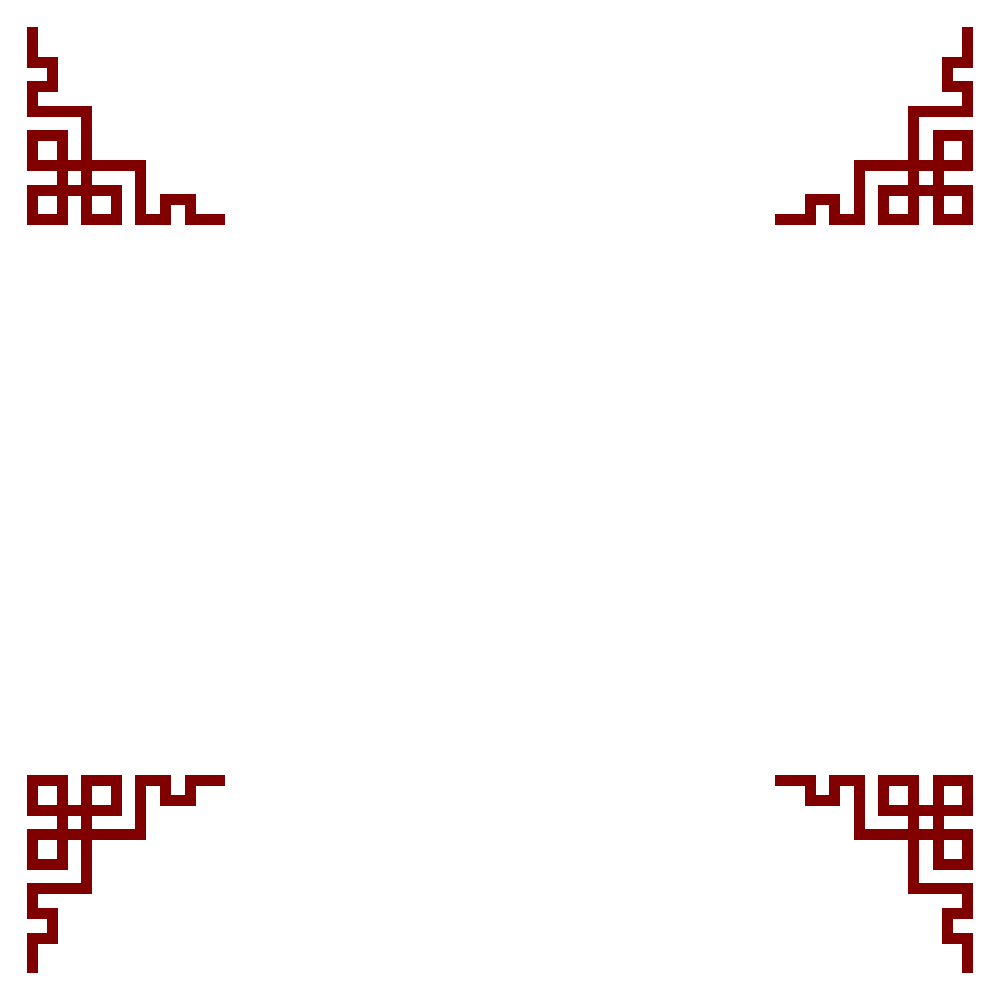
\begin{tikzpicture}[color=Maroon,
        every node/.style={inner sep=0pt}]
        \node[minimum size=12cm](vecbox){%
            \begin{minipage}{\textwidth}
            \centering
        \BODY
    \end{minipage}};
        \node[anchor=north west] at (vecbox.north west)
        {\pgfornament[width=2.5cm,symmetry=h]{3}};
        \node[anchor=north east] at (vecbox.north east)
        {\pgfornament[width=2.5cm,symmetry=c]{3}};
        \node[anchor=south west] at (vecbox.south west)
        {\pgfornament[width=2.5cm,symmetry=none]{3}};
        \node[anchor=south east] at (vecbox.south east)
        {\pgfornament[width=2.5cm,symmetry=v]{3}};
        \end{tikzpicture}
}

\newcommand{\seq}{\texttt{;}}
\newcommand{\paral}{\textbardbl}
\newcommand{\sat}{$\top$}
\newcommand{\unsat}{$\bot$}
\newcommand{\fast}{\texttt{24}}
\newcommand{\inc}{inc}
\newcommand{\uc}{uc}
\newcommand{\mv}{mv}
\newcommand{\cloud}{cloud}
\newcommand{\paralTrack}{parallel}
%\newcommand{\all}{{\footnotesize (\seq,\paral,\sat,\unsat,\fast,\inc,\uc\seq,\uc\paral,\mv)}}
\newcommand{\withtrack}[2]{\textsc{#1}{{\footnotesize (#2)}}}

\newcommand{\MakeOnePage}[6]{
    {\centering
    {

    \begin{minipage}{\textwidth}
    \centering

    
\begin{tikzpicture}
      \node [circular drop shadow={shadow scale=1.05},
             decorate, decoration=zigzag,
             fill=blue!20,draw,thick,circle,text width=3.5cm,align=center,xshift=2cm]
              {\large\textbf{SMT-COMP\\ 2024}};
    \end{tikzpicture}
    \end{minipage}

    \begin{myframe}

    \textcolor{red!10!black!90}
    {\Huge #1}\\

    \textcolor{green!10!black!90}{
    \large In honor of the results achieved in the SMT-competition}

    \medskip
    \ifstrempty{#2}{}{
    \textcolor{red!30!black!90}
    {\textit{Overall Winner}}


    \textcolor{black}{\large #2}

     \medskip
    }

    \ifstrempty{#3}{}{
    \textcolor{red!30!black!90} {\textit{Winner of the Division#5}}

     \textcolor{black}{\large#3}

     \medskip
    }

    \ifstrempty{#4}{}{
     \textcolor{red!30!black!90}  {\textit{Winner of the Logic#6
      \ifstrempty{#3}{}{(where it did not win the corresponding division)}}}

     \textcolor{black}{\large #4}
    }
    \vspace{2mm}


    \vspace{1cm}

    {\color{blue!40!black}
%    \scalebox{.7}{
    {\tiny
    \begin{tabular}{ccccc}
        \includegraphics[scale=0.25,trim=1.5cm 2.75cm 0pt 0pt]{FB-signature.png} &&
        \includegraphics[trim=0pt 0.20cm 0pt 0pt]{MB-Signature.png} &&
        \includegraphics[scale=0.4,trim=1.5pt 2.75cm 0pt 0pt]{MJ-Signature.png} \\
    \cline{1-1}
    \cline{3-3}
    \cline{5-5}
    \\ \
    François Bobot & & Martin Bromberger & & Martin Jon\'{a}\v{s} \\
    Organizer & & Chair & & Organizer \\
    \end{tabular}
    }}
    \end{myframe}
    }}

}

\begin{document}

\TileWallPaper{4cm}{2cm}{tiling.png}

\MakeOnePage{Algaroba}{}{\withtrack{QF\_Datatypes}{\seq,\paral,\fast}}{\withtrack{QF\_DT}{\sat}}{}{}
\newpage
\MakeOnePage{Amaya}{}{}{\withtrack{NIA}{\fast}}{}{}
\newpage
\MakeOnePage{Bitwuzla}{\withtrack{Biggest Lead}{\inc}}{\withtrack{Bitvec}{\sat}, \withtrack{Equality\_MachineArith}{\inc,\uc}, \withtrack{FPArith}{\seq,\paral,\sat,\unsat,\fast,\inc}, \withtrack{QF\_ADT\_BitVec}{\mv}, \withtrack{QF\_Bitvec}{\seq,\paral,\unsat,\fast,\inc}, \withtrack{QF\_Equality\_Bitvec}{\seq,\paral,\sat,\unsat,\inc}, \withtrack{QF\_FPArith}{\seq,\paral,\sat,\unsat,\fast,\inc,\uc}}{\withtrack{ABVFP}{\sat}, \withtrack{AUFBV}{\seq,\paral,\sat,\unsat,\fast}, \withtrack{AUFBVFP}{\seq,\paral,\sat,\unsat,\fast}, \withtrack{BVFPLRA}{\uc}, \withtrack{QF\_ABV}{\uc\textsuperscript\seq}, \withtrack{QF\_ABVFP}{\mv}, \withtrack{QF\_BVFPLRA}{\mv}, \withtrack{QF\_FPLRA}{\mv}, \withtrack{QF\_UFBV}{\fast}, \withtrack{UFBV}{\fast}}{s}{s}
\newpage
\MakeOnePage{COLIBRI}{}{}{\withtrack{QF\_ABVFPLRA}{\unsat}, \withtrack{QF\_FP}{\fast}, \withtrack{QF\_FPLRA}{\unsat,\fast}}{}{s}
\newpage
\MakeOnePage{cvc5}{\withtrack{Biggest Lead}{\seq,\paral,\sat,\unsat,\fast}, \withtrack{Largest Contribution}{\seq,\paral,\sat,\unsat,\fast}}{\withtrack{Arith}{\seq,\paral,\unsat,\inc}, \withtrack{Bitvec}{\seq,\paral,\unsat,\inc,\uc}, \withtrack{Equality}{\seq,\paral,\sat,\unsat,\fast,\inc}, \withtrack{Equality\_LinearArith}{\seq,\paral,\sat,\unsat,\fast,\inc}, \withtrack{Equality\_MachineArith}{\seq,\paral,\sat,\unsat,\fast}, \withtrack{Equality\_NonLinearArith}{\seq,\paral,\sat,\unsat,\fast,\inc}, \withtrack{FPArith}{\uc}, \withtrack{QF\_Datatypes}{\sat,\uc}, \withtrack{QF\_Equality\_LinearArith}{\uc\textsuperscript\paral}, \withtrack{QF\_Equality\_NonLinearArith}{\unsat,\inc,\uc\textsuperscript\seq,\mv}, \withtrack{QF\_FPArith}{\mv}, \withtrack{QF\_LinearIntArith}{\unsat}, \withtrack{QF\_LinearRealArith}{\unsat}, \withtrack{QF\_NonLinearRealArith}{\unsat}, \withtrack{QF\_Strings}{\uc}}{\withtrack{ANIA}{\uc}, \withtrack{AUFBV}{\uc\textsuperscript\paral}, \withtrack{AUFBVDTLIA}{\uc}, \withtrack{AUFBVDTNIRA}{\uc}, \withtrack{AUFDTLIRA}{\uc\textsuperscript\seq}, \withtrack{AUFFPDTNIRA}{\uc}, \withtrack{AUFLIRA}{\uc\textsuperscript\seq}, \withtrack{AUFNIA}{\uc\textsuperscript\paral}, \withtrack{BVFPLRA}{\unsat}, \withtrack{FP}{\fast}, \withtrack{LIA}{\sat,\fast}, \withtrack{NIA}{\sat}, \withtrack{QF\_AUFLIA}{\inc,\uc\textsuperscript\seq}, \withtrack{QF\_AX}{\mv}, \withtrack{QF\_BVFP}{\inc}, \withtrack{QF\_FP}{\sat,\uc}, \withtrack{QF\_IDL}{\uc}, \withtrack{QF\_LIA}{\mv}, \withtrack{QF\_SNIA}{\seq,\paral,\sat,\fast}, \withtrack{QF\_UFBVDT}{\seq,\paral,\unsat,\fast,\uc,\mv}, \withtrack{QF\_UFDT}{\seq,\paral,\mv}, \withtrack{QF\_UFDTLIRA}{\seq,\paral,\sat,\unsat,\fast,\uc\textsuperscript\seq,\mv}, \withtrack{QF\_UFDTNIA}{\seq,\paral,\sat,\fast}, \withtrack{QF\_UFFPDTNIRA}{\seq,\paral,\sat,\unsat,\fast}, \withtrack{QF\_UFLRA}{\inc,\uc\textsuperscript\seq}, \withtrack{UFDT}{\uc\textsuperscript\seq}, \withtrack{UFDTLIA}{\uc\textsuperscript\seq}, \withtrack{UFDTNIA}{\uc\textsuperscript\seq}, \withtrack{UFFPDTNIRA}{\uc}, \withtrack{UFIDL}{\uc\textsuperscript\seq}, \withtrack{UFLRA}{\uc}, \withtrack{UFNIRA}{\uc\textsuperscript\seq}}{s}{s}
\newpage
\MakeOnePage{iProver v3.9}{}{}{\withtrack{ALIA}{\paral,\unsat}, \withtrack{UF}{\fast}, \withtrack{UFNIRA}{\seq,\unsat}}{}{s}
\newpage
\MakeOnePage{OpenSMT}{}{\withtrack{QF\_Equality}{\mv}, \withtrack{QF\_Equality\_LinearArith}{\unsat,\mv}, \withtrack{QF\_LinearIntArith}{\seq,\paral,\mv}, \withtrack{QF\_LinearRealArith}{\seq,\paral,\sat,\inc,\mv}}{\withtrack{QF\_LIA}{\sat}, \withtrack{QF\_LRA}{\unsat,\fast}, \withtrack{QF\_UFIDL}{\seq,\paral,\sat}}{s}{s}
\newpage
\MakeOnePage{SMT-RAT}{}{\withtrack{QF\_NonLinearRealArith}{\mv}}{\withtrack{NRA}{\seq,\paral,\unsat,\fast}}{}{}
\newpage
\MakeOnePage{SMTInterpol}{\withtrack{Biggest Lead}{\uc,\mv}}{\withtrack{Arith}{\uc}, \withtrack{Equality}{\uc\textsuperscript\paral}, \withtrack{Equality\_LinearArith}{\uc}, \withtrack{Equality\_NonLinearArith}{\uc}, \withtrack{QF\_ADT\_LinArith}{\mv}, \withtrack{QF\_Datatypes}{\mv}, \withtrack{QF\_Equality\_LinearArith}{\seq,\paral,\sat,\inc,\uc\textsuperscript\seq}, \withtrack{QF\_Equality\_NonLinearArith}{\uc\textsuperscript\paral}, \withtrack{QF\_NonLinearIntArith}{\inc,\uc}, \withtrack{QF\_NonLinearRealArith}{\uc}}{\withtrack{ALIA}{\sat}, \withtrack{ANIA}{\seq,\paral,\sat,\unsat,\fast}, \withtrack{QF\_ALIA}{\uc\textsuperscript\paral}, \withtrack{QF\_ANIA}{\unsat,\fast,\inc,\uc\textsuperscript\seq,\mv}, \withtrack{QF\_AUFNIA}{\sat,\uc\textsuperscript\seq,\mv}, \withtrack{QF\_LIA}{\unsat}, \withtrack{QF\_LIRA}{\uc\textsuperscript\paral}, \withtrack{QF\_UF}{\uc\textsuperscript\paral}, \withtrack{QF\_UFBVDT}{\sat}, \withtrack{QF\_UFDTLIA}{\unsat,\fast,\uc\textsuperscript\paral}, \withtrack{QF\_UFDTNIA}{\uc\textsuperscript\seq,\mv}, \withtrack{QF\_UFLIA}{\unsat,\mv}, \withtrack{QF\_UFNRA}{\uc\textsuperscript\seq}, \withtrack{UFIDL}{\sat}, \withtrack{UFLIA}{\sat}}{s}{s}
\newpage
\MakeOnePage{STP}{}{\withtrack{QF\_Bitvec}{\sat,\mv}}{}{}{}
\newpage
\MakeOnePage{Yices2}{\withtrack{Largest Contribution}{\uc,\mv}}{\withtrack{Equality}{\uc\textsuperscript\seq}, \withtrack{QF\_Bitvec}{\uc}, \withtrack{QF\_Equality}{\seq,\paral,\sat,\unsat,\fast,\inc,\uc}, \withtrack{QF\_Equality\_Bitvec}{\fast,\uc,\mv}, \withtrack{QF\_Equality\_Bitvec\_Arith}{\inc}, \withtrack{QF\_Equality\_LinearArith}{\fast}, \withtrack{QF\_Equality\_NonLinearArith}{\seq,\paral,\sat,\fast}, \withtrack{QF\_LinearIntArith}{\fast,\inc,\uc}, \withtrack{QF\_LinearRealArith}{\fast,\uc}, \withtrack{QF\_NonLinearIntArith}{\fast,\mv}, \withtrack{QF\_NonLinearRealArith}{\fast}}{\withtrack{QF\_ALIA}{\unsat}, \withtrack{QF\_AUFLIA}{\seq,\paral,\sat,\unsat}, \withtrack{QF\_AUFNIA}{\unsat}, \withtrack{QF\_IDL}{\mv}, \withtrack{QF\_LIRA}{\sat,\mv}, \withtrack{QF\_RDL}{\seq,\paral,\sat,\unsat,\mv}, \withtrack{QF\_UFLIA}{\inc,\uc\textsuperscript\seq}, \withtrack{QF\_UFLRA}{\seq,\paral,\sat,\unsat,\mv}, \withtrack{QF\_UFNRA}{\unsat,\mv}, \withtrack{UF}{\uc\textsuperscript\paral}}{s}{s}
\newpage
\MakeOnePage{YicesQS}{}{\withtrack{Arith}{\sat,\fast}, \withtrack{Bitvec}{\fast}}{\withtrack{LRA}{\seq,\paral,\unsat}}{s}{}
\newpage
\MakeOnePage{Z3-alpha}{}{\withtrack{QF\_Datatypes}{\unsat}, \withtrack{QF\_LinearIntArith}{\sat}, \withtrack{QF\_NonLinearIntArith}{\seq,\paral,\sat,\unsat}, \withtrack{QF\_NonLinearRealArith}{\seq,\paral,\sat}}{\withtrack{QF\_AUFBV}{\unsat}, \withtrack{QF\_IDL}{\seq,\paral,\unsat}, \withtrack{QF\_LIRA}{\seq,\paral,\unsat}, \withtrack{QF\_NIRA}{\fast}}{s}{s}
\newpage
\MakeOnePage{Z3-Noodler}{}{\withtrack{QF\_Strings}{\seq,\paral,\sat,\unsat,\fast}}{}{}{}
\newpage


\end{document}
